\section{Sezione Introduttiva}

\subsection{Team Members}
I membri del gruppo sono:
\begin{itemize} 
    \item Giulio Gualtiero, 234656, GitHub: \href{https://github.com/GiulioGualtiero}{GiulioGualtiero}
    \item Jago Revrenna, 235081, GitHub: \href{https://github.com/jagorev}{jagorev}
    \item Tommaso Onori, 234893, GitHub: \href{https://github.com/TommasoOnori}{TommasoOnori}
\end{itemize}

\subsection{Project Idea}
Il progetto prevede lo sviluppo di un sistema intelligente per la gestione dei rifiuti a Trento, composto da un'app mobile per i cittadini e una web app per il Comune. L'obiettivo è ottimizzare la raccolta e lo smaltimento tramite notifiche, segnalazioni e monitoraggio in tempo reale, migliorando l'efficienza e la sostenibilità del servizio.
\subsection{External References}
Collegamenti a risorse esterne:
\begin{itemize}
    \item Repository GitHub: \href{https://github.com/jagorev/EcoTrack}{EcoTrack}
    \item Swagger HUB: \href{ https://app.swaggerhub.com/apis-docs/universityoftrento/EcoTrackAPI/1.0.0#/}{EcoTrack}
    \item Link a Deployment con Render: \href{https://ecotrack-6pp4.onrender.com/}{Web App - EcoTrack}

Account di test disponibili (uno per classe di utenza):

\begin{itemize}
    \item \textbf{Credenziali Admin}: AdminProf , A1i5tarC0ckburn!
\end{itemize}

\item L'APK della Mobile App è disponibile su GitHub al seguente link: \href{https://github.com/jagorev/EcoTrack/tree/main/apk%20mobile%20app}{EcoTrack APK}


    
\end{itemize}

\section{Sezione Generale}
\subsection{Strategia di Branching}
Abbiamo scelto il \textbf{Feature Branch Workflow} come strategia di branching poiché, essendo il nostro team composto da soli tre membri, risulta semplice ed efficace: ci consente di lavorare in parallelo su funzionalità diverse senza dover affrontare continuamente conflitti di merge. \\Nel caso del nostro progetto, questo approccio ci aiuta a mantenere il branch master stabile e sempre pronto per l’integrazione, rendendo allo stesso tempo più semplice la gestione e la revisione del codice attraverso pull request pulite e dettagliate per ogni nuova funzionalità o correzione di bug. 
\\Inoltre, tale approccio può essere facilmente integrato, all’occorrenza, con una strategia più strutturata come il \textbf{Gitflow Workflow}, qualora il progetto dovesse crescere in complessità.

\subsection{Product Backlog}
È possibile visualizzare il product backlog di EcoTrack al seguente link: \href{https://docs.google.com/spreadsheets/d/124BGyj-mUSipfd_NPPftBozjqdOnjI-apbYR-fjCgLY/edit?usp=sharing}{EcoTrack - Product Backlog}.
\begin{figure}[H]
    \centering
    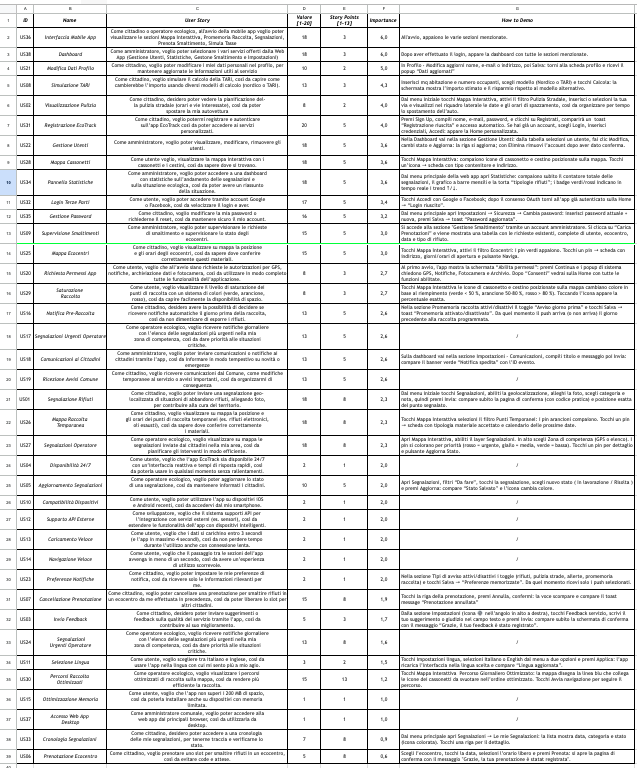
\includegraphics[width=1\linewidth]{D3-G1//Img/Screenshot Product Backlog.png}
    \caption{Product Backlog Overview}
    \label{fig:enter-label}
\end{figure}

\subsection{Definition of Done}
\begin{longtable}{p{3cm}p{11cm}}
\toprule
Categoria & Criterio \\
\midrule
\endfirsthead
\toprule
Categoria & Criterio \\
\midrule
\endhead
Qualità del Codice & Codice conforme agli standard di stile. Nessun errore dev'essere presente. \\
Test e Validazione & Validazione su ambiente di sviluppo o staging completata. \\
Documentazione & Documentazione tecnica aggiornata. Commenti chiari all'interno del codice dove necessario. \\
Sicurezza & Gestione sicura dei dati utente e delle credenziali. \\
Revisione & Code review completata e approvata da almeno un altro membro del team. Correzione di tutte le osservazioni emerse. \\
Deployabilità & Funzionalità integrabile nel ramo principale senza conflitti. Pronta per la release successiva o incremento sprint. \\
\bottomrule
\end{longtable}

\section{Sezione Sprint}
\subsection{Obiettivo dello Sprint}
L’obiettivo del secondo sprint è stato quello di perfezionare ulteriormente l’applicazione EcoTrack, ampliando e consolidando le funzionalità di base già implementate nella prima versione, con un focus specifico sullo sviluppo e il miglioramento della versione mobile.

 Il team si è concentrato sull’implementazione di 12 nuove user stories, selezionate tra quelle prioritarie, puntando sia sull’aggiunta di nuove funzionalità che sull’ottimizzazione del codice esistente per migliorarne l’affidabilità, le prestazioni e la stabilità complessiva.


 Questo sprint ha contribuito a rendere la mobile app e la web app più completa e coerente, avvicinandola a una versione quasi definitiva, pronta per essere testata in scenari reali e per accogliere componenti avanzati nei successivi cicli di sviluppo. 

\subsection{Sprint Planning}
\subsubsection{Sprint Backlog}
È possibile visualizzare il secondo sprint backlog di EcoTrack al seguente link: \href{https://docs.google.com/spreadsheets/d/1UYSNiXJVttFC2hsekku7MCvBMyUbau9QfrwKCSSBOCM/edit?usp=sharing}{EcoTrack - Sprint Backlog}.

\begin{figure} [H]
    \centering
    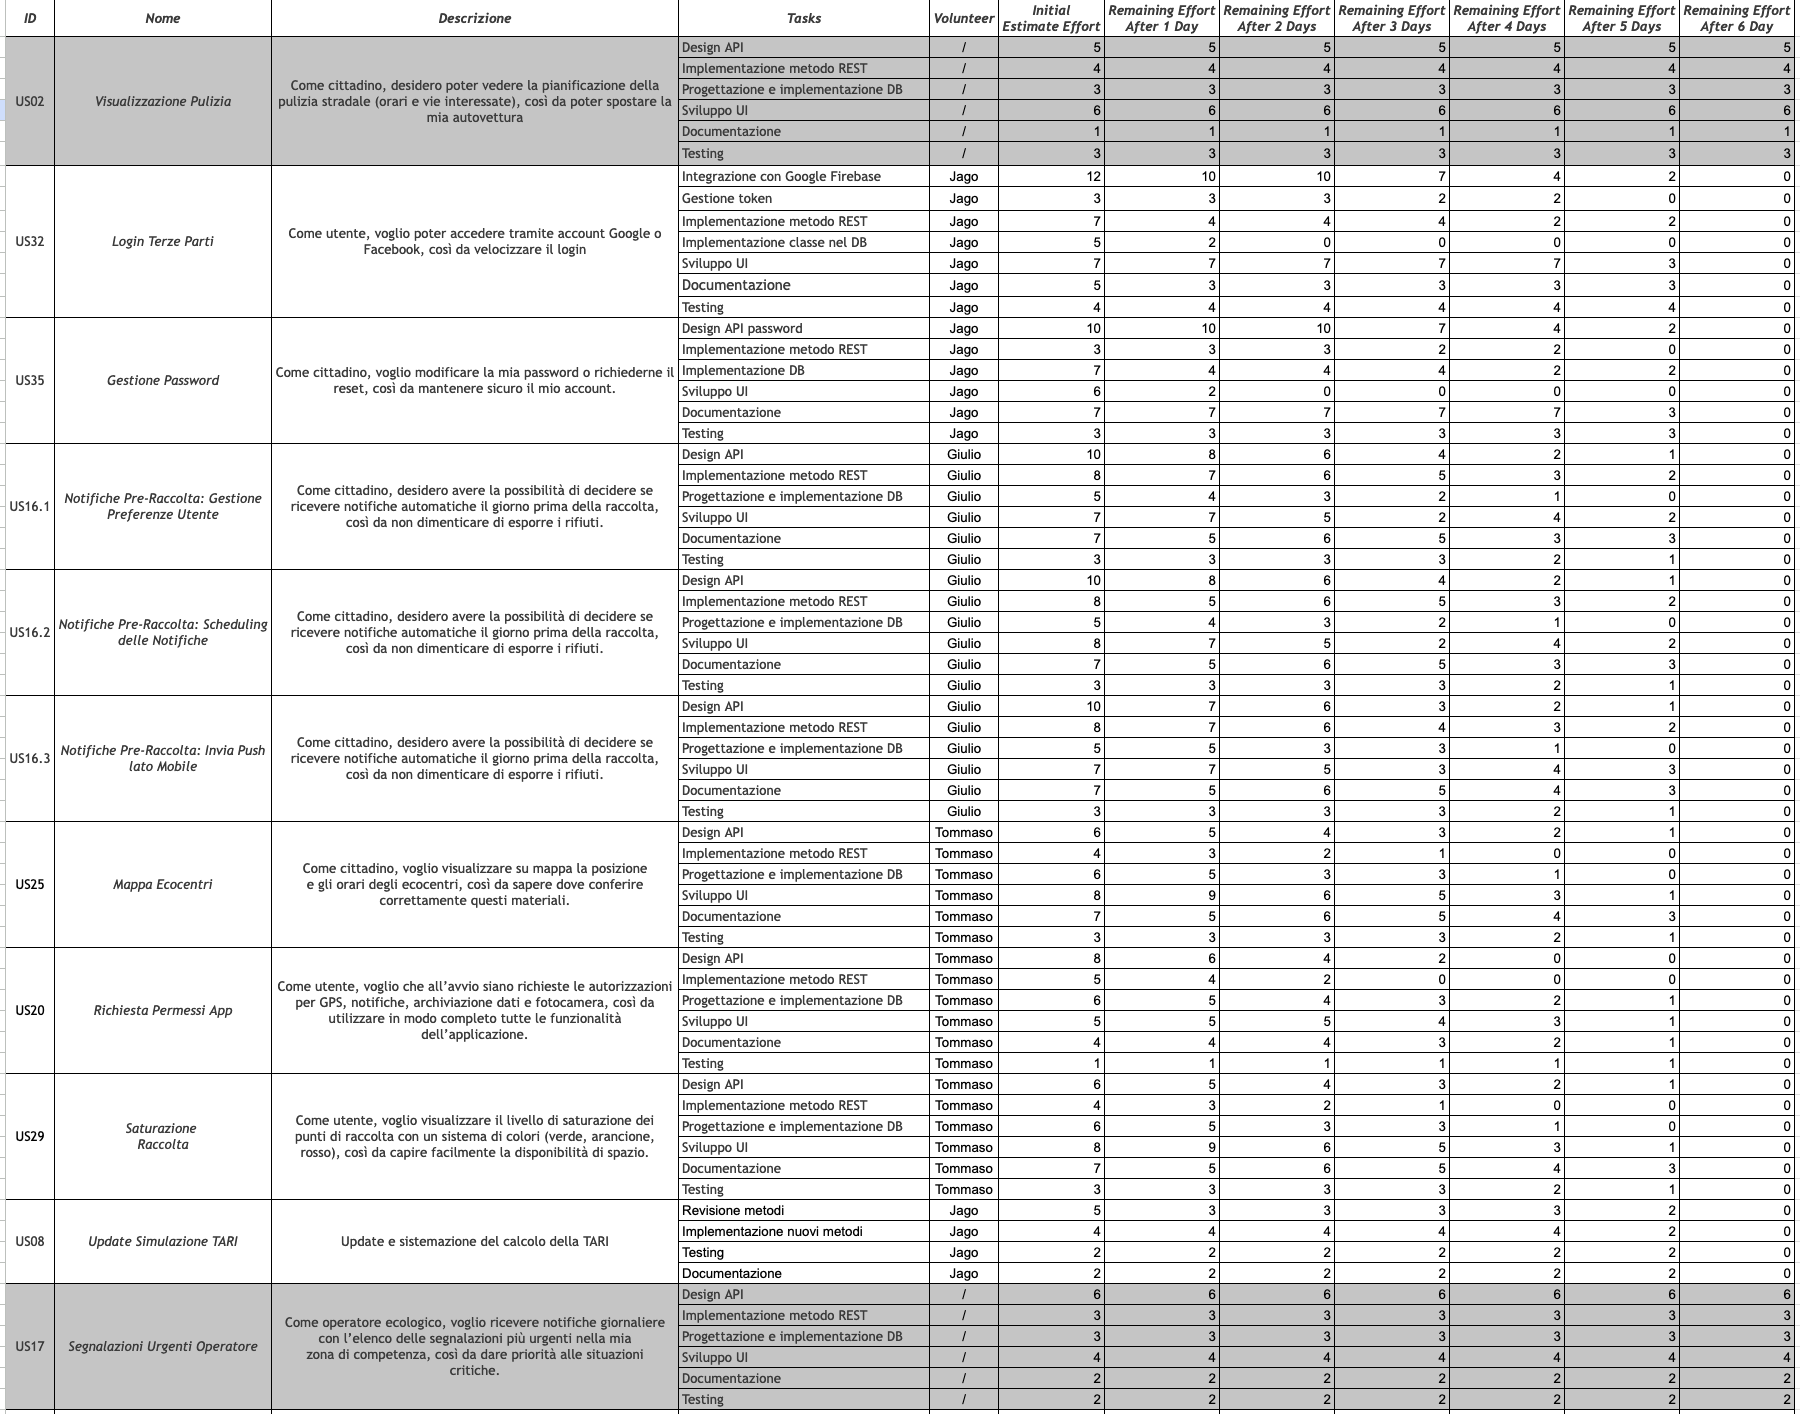
\includegraphics[width=1\linewidth]{D4-G1//Img/Screenshot 2025-06-10 at 14.14.02.png}
    \label{fig:enter-label}
\end{figure}

\begin{figure} [H]
    \centering
    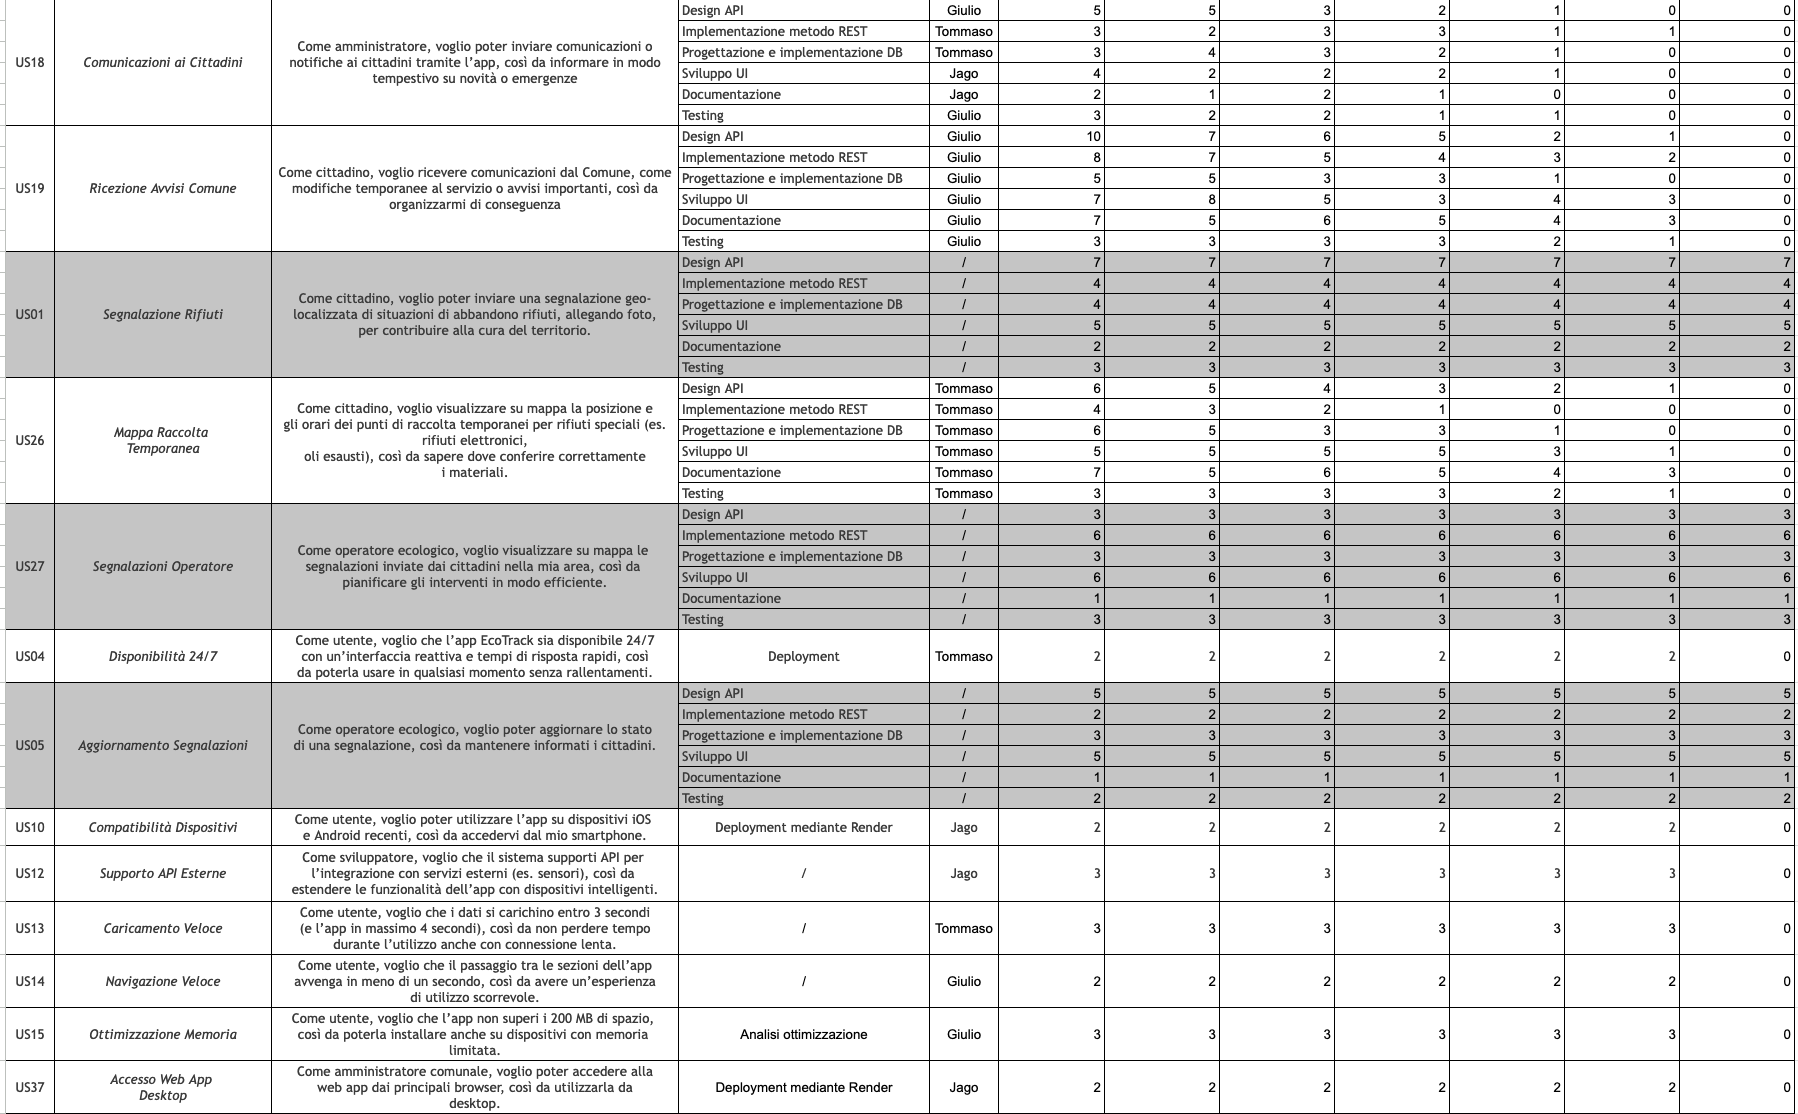
\includegraphics[width=1\linewidth]{D4-G1//Img/Screenshot 2025-06-10 at 14.14.44.png}
    \caption{Sprint Backlog Overview. Le user stories evidenziate in grigio non sono state implementate.}
    \label{fig:enter-label}
\end{figure}

\subsubsection{Burndown Chart}
\begin{figure} [H]
    \centering
    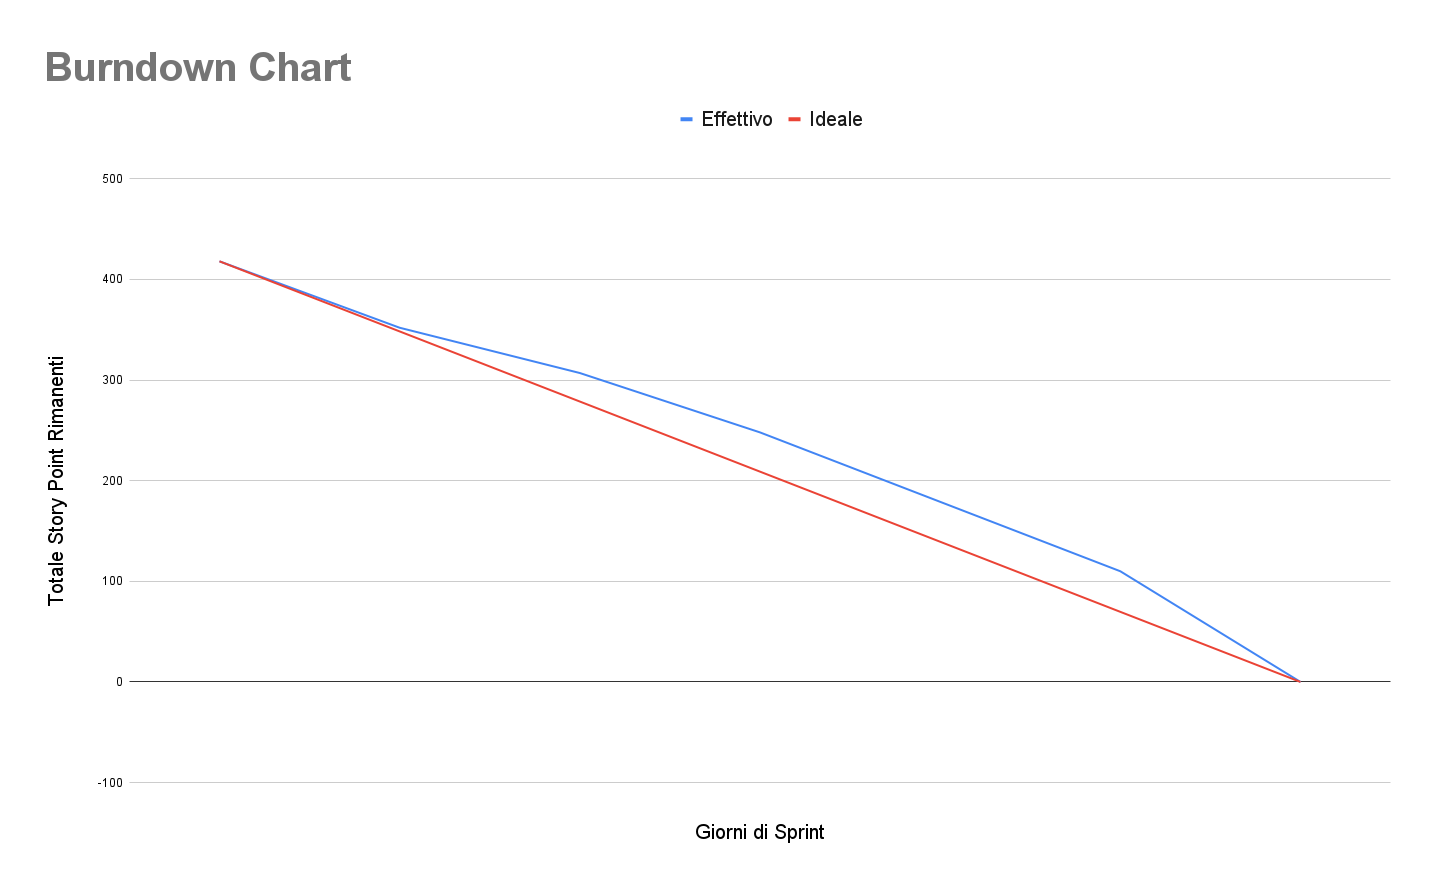
\includegraphics[width=1\linewidth]{D4-G1//Img/Burndown Chart - Sprint 2.png}
    \caption{L'andamento effettivo non tiene in considerazione le user stories non implementate.}
    \label{fig:enter-label}
\end{figure}

\subsection{Test Cases}
È possibile visualizzare i casi di test di EcoTrack al seguente link: \href{https://docs.google.com/spreadsheets/d/19TjIHKf8wvDxEds9eg8yDFcew4lJyGeI82jz5czIyQI/edit?usp=sharing}{EcoTrack - Test Cases}.

Sono stati effettuati anche alcuni test sulle API mediante l'utilizzo del framework di testing Jest. Qui di seguito sono riportati i risultati di 28 test. I file di test in questione sono situati nella cartella \texttt{tests} della repository GitHub.
\begin{figure}[H]
    \centering
    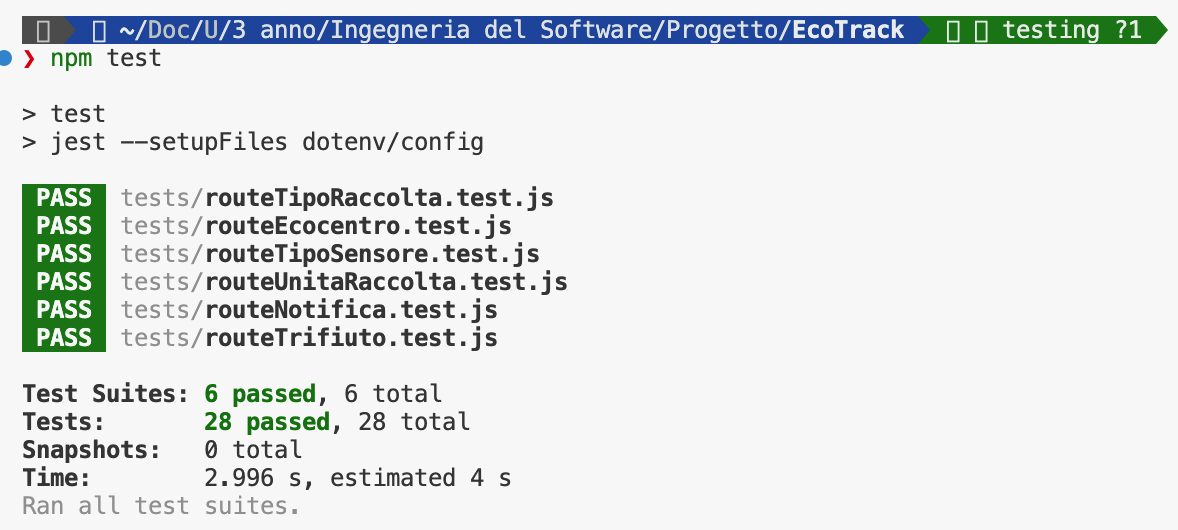
\includegraphics[width=1\linewidth]{D4-G1//Img/Testing_Jest.png}
    \caption{Risultati dei test effettuati con Jest}
    \label{fig:enter-label}
\end{figure}

\begin{figure}[H]
    \centering
    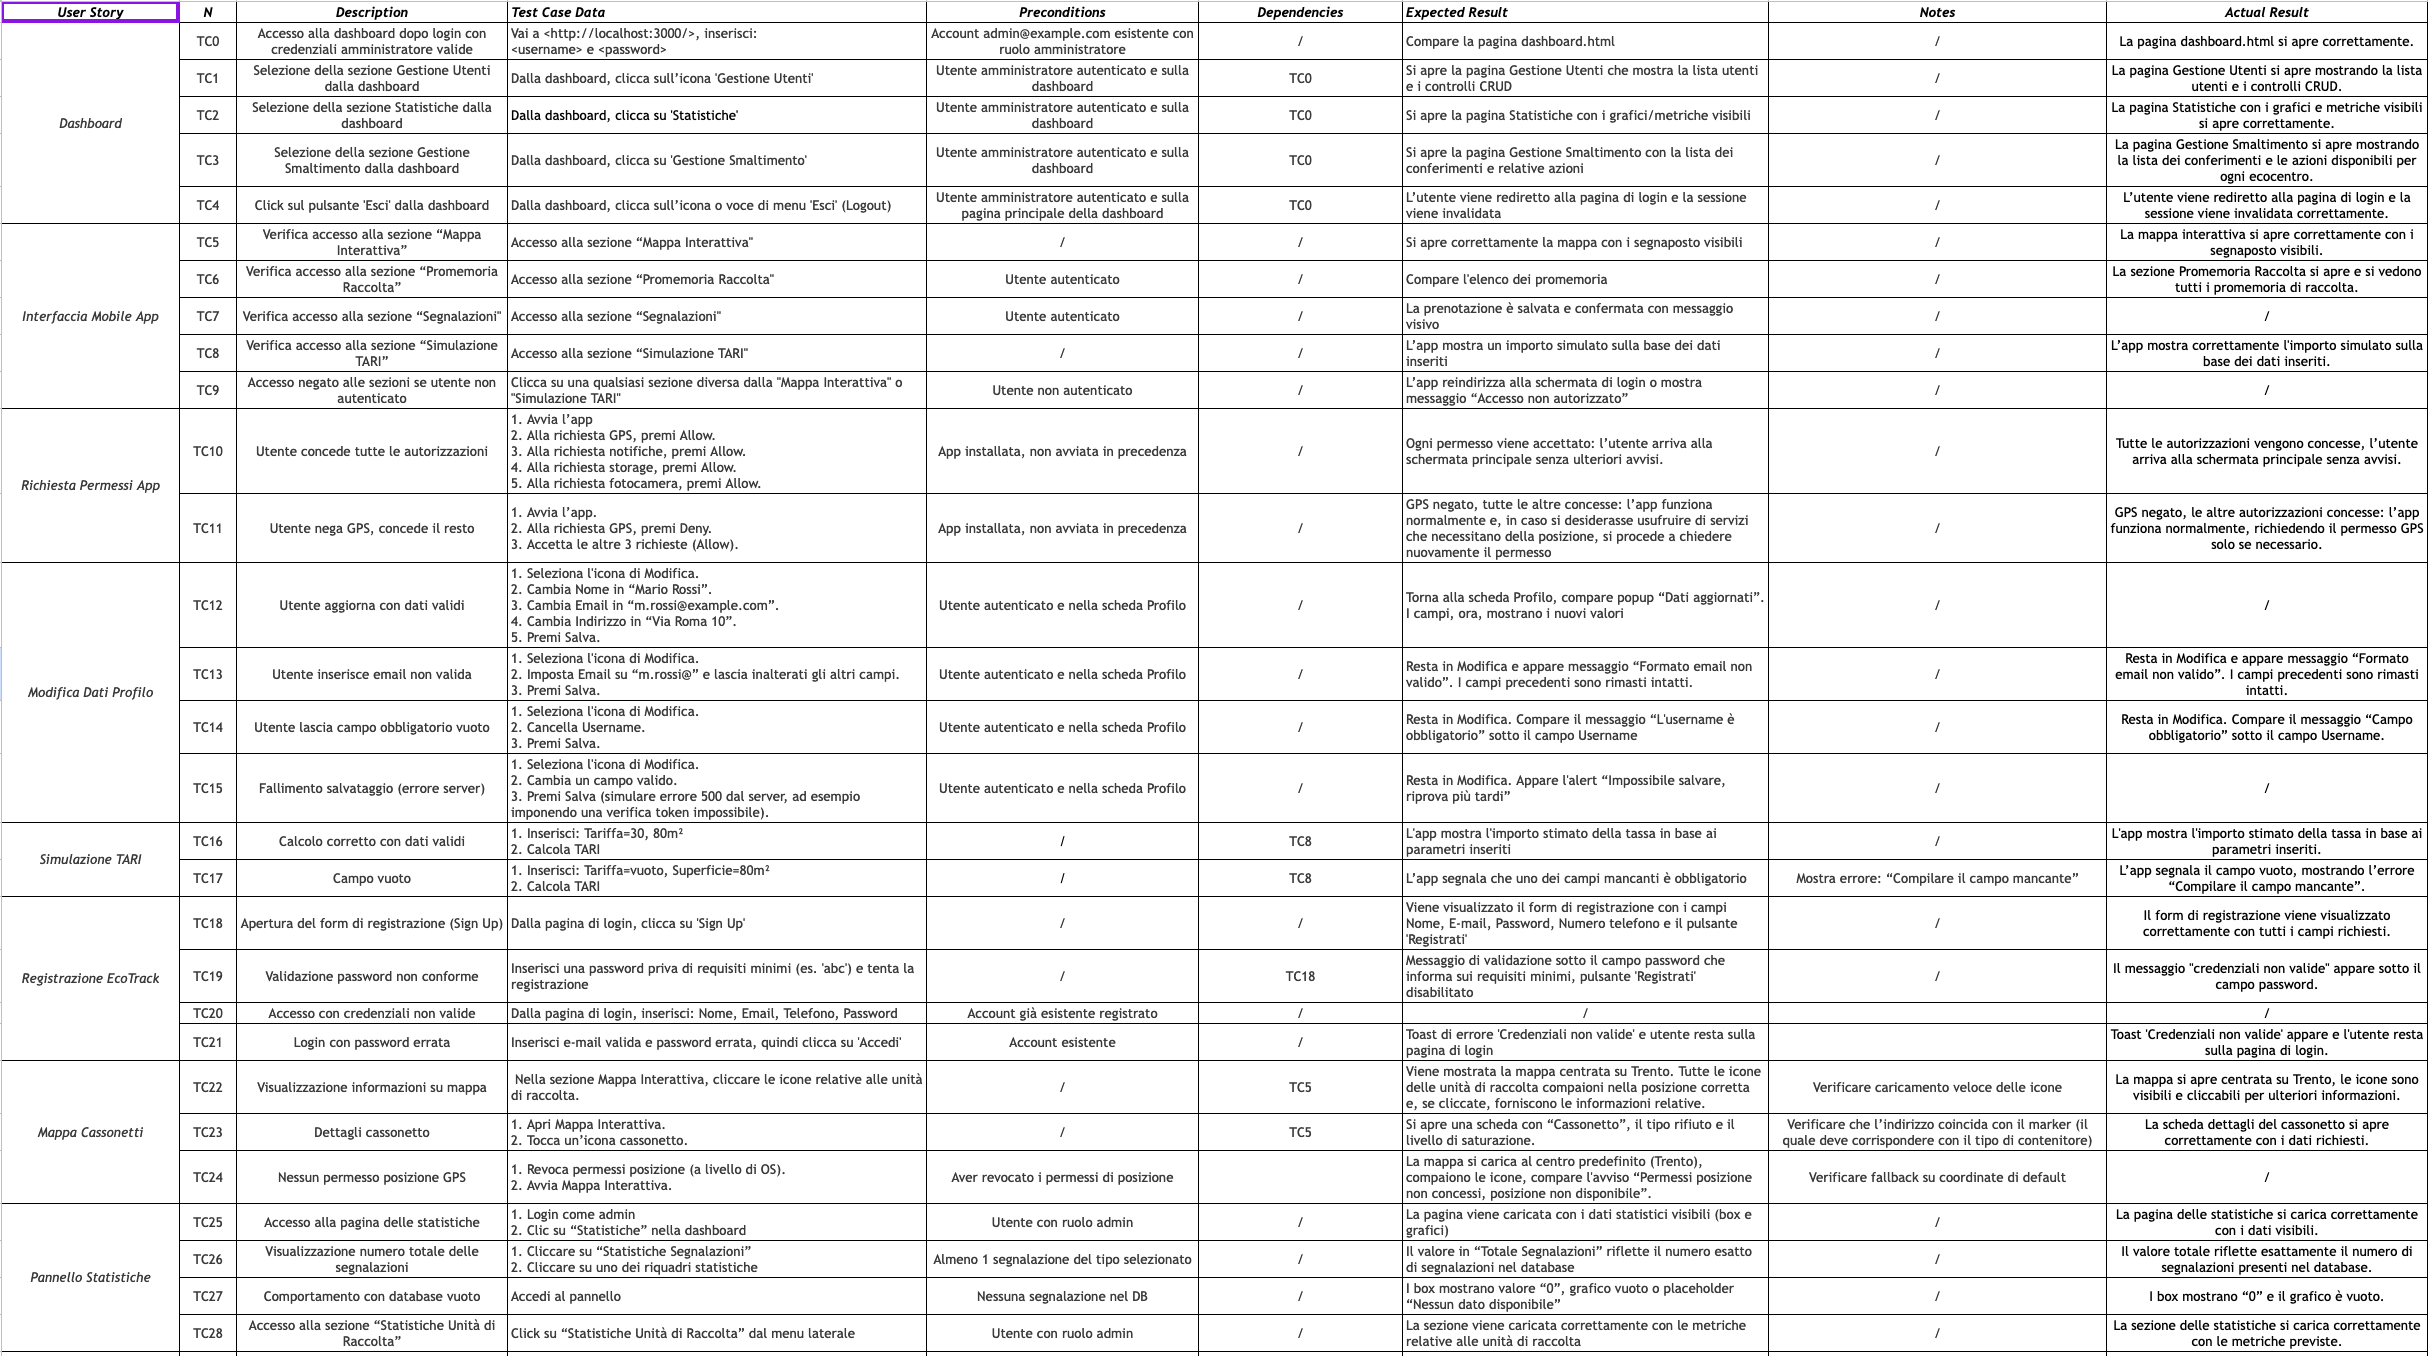
\includegraphics[width=1\linewidth]{D4-G1//Img/Screenshot 2025-06-10 at 18.19.58.png}
    \label{fig:enter-label}
\end{figure}
\begin{figure}[H]
    \centering
    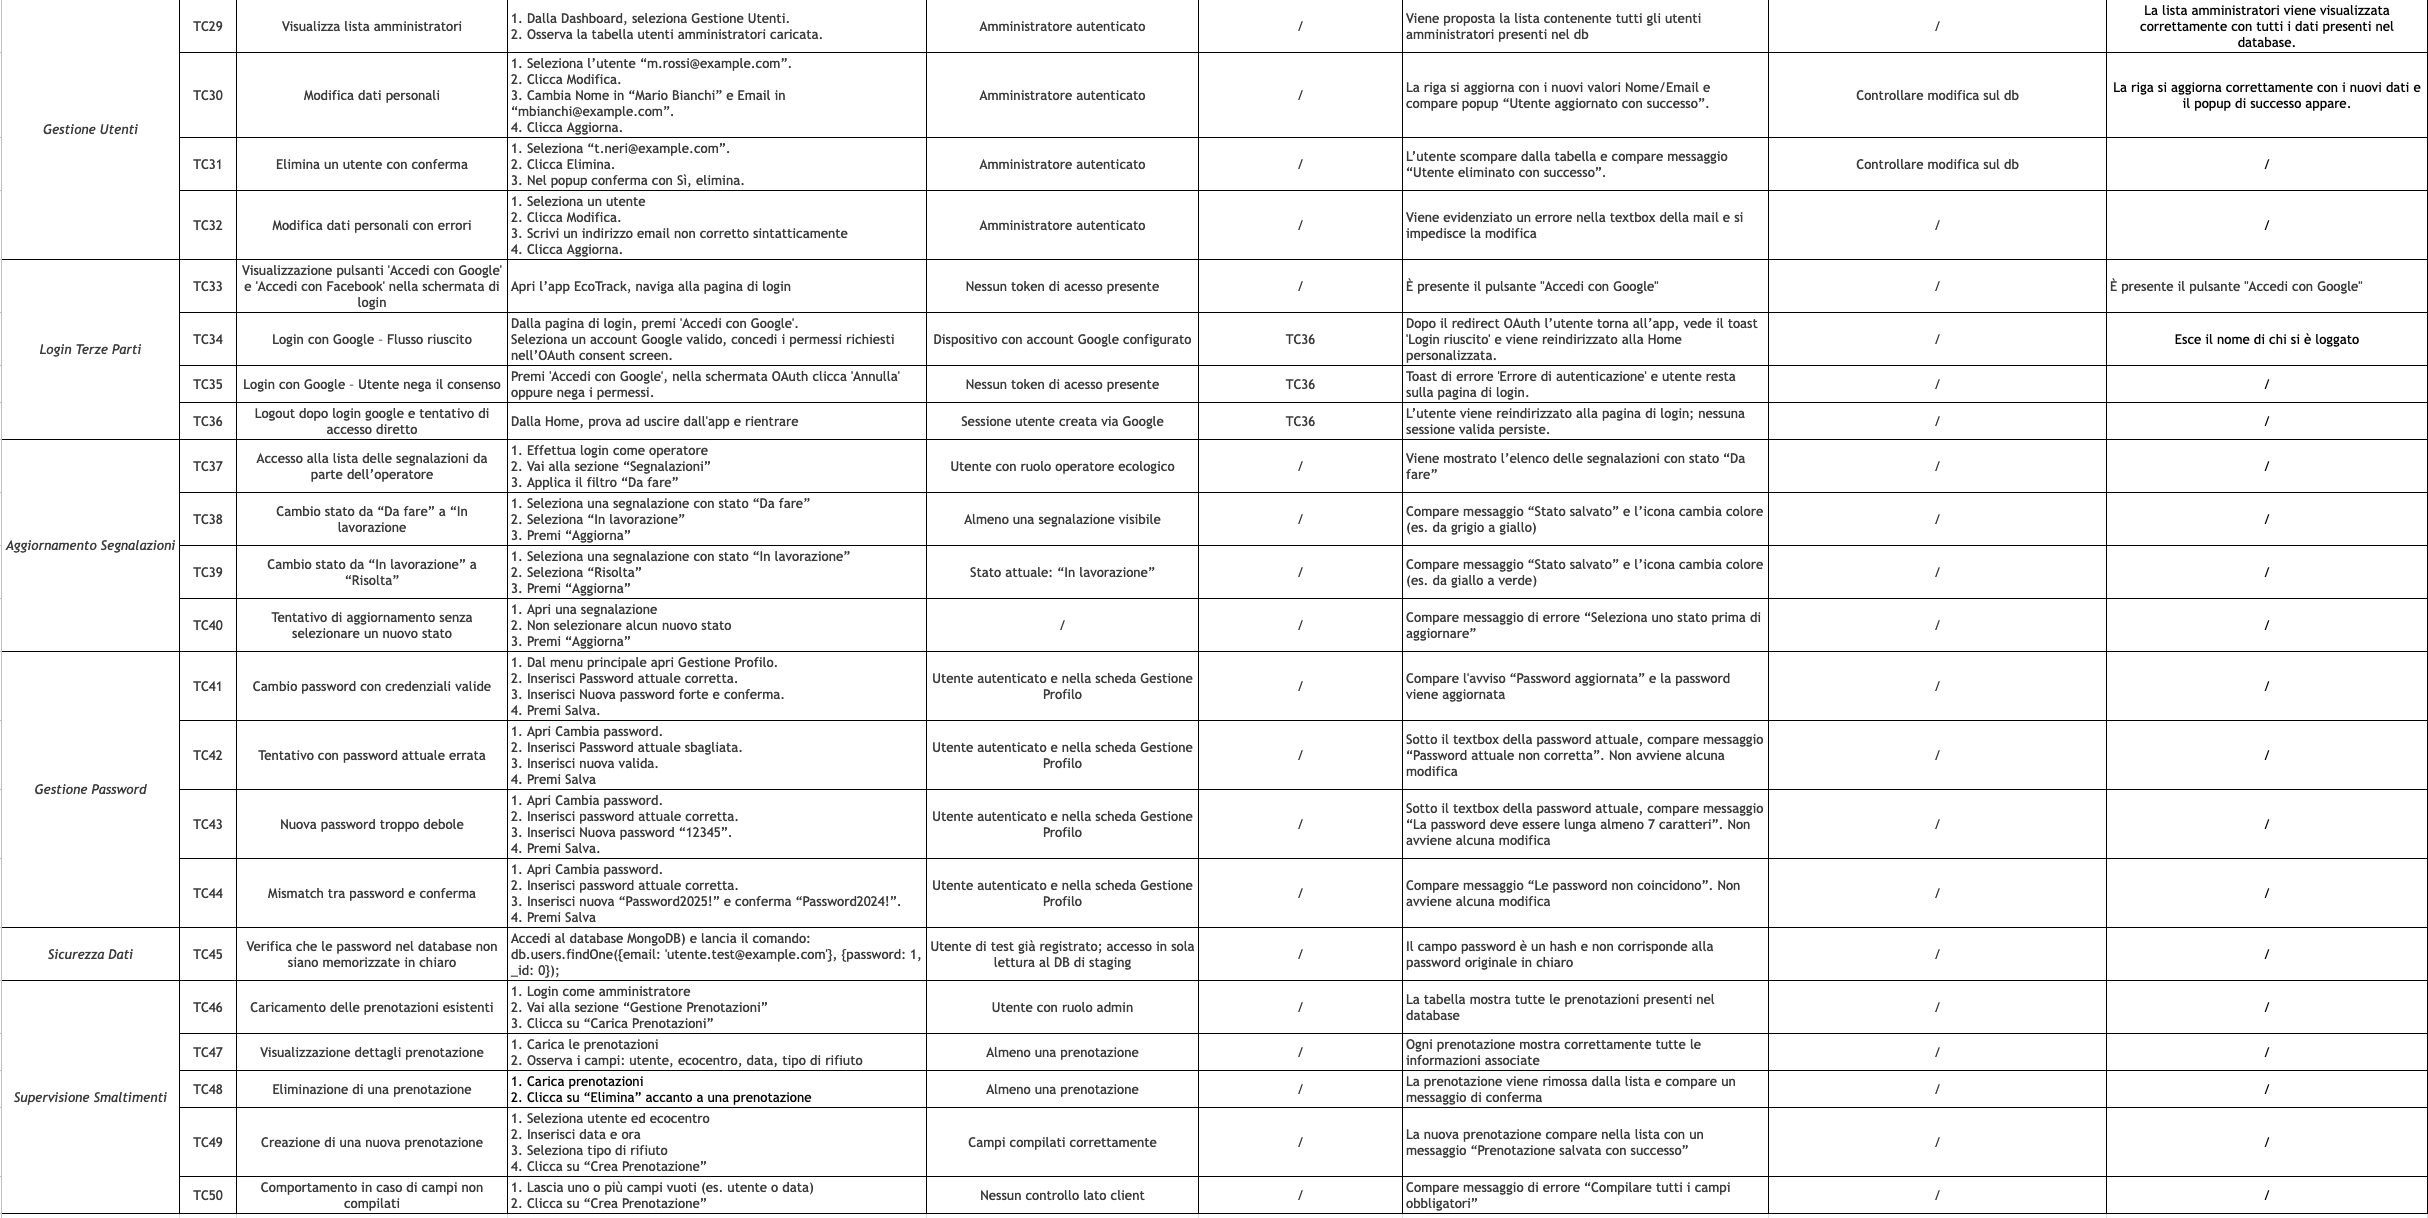
\includegraphics[width=1\linewidth]{D4-G1//Img/Screenshot 2025-06-10 at 18.20.20.png}
    \caption{Tabella di Test Cases (screenshot)}
    \label{fig:enter-label}
\end{figure}


\subsection{Sprint Review}
Durante questo sprint, il team di sviluppo composto da \textbf{Giulio}, \textbf{Jago} e \textbf{Tommaso} ha lavorato su diverse aree chiave del progetto EcoTrack. Particolare attenzione è stata dedicata allo sviluppo e perfezionamento del sistema di \textbf{gestione notifiche}, sia lato \textbf{backend} che \textbf{frontend}. Parallelamente, sono stati portati avanti l’integrazione del \textbf{login} tramite \textbf{Firebase}, la\textbf{ gestione interattiva della mappa} e le attività di \textbf{deployment}. Lo sprint si è concluso con il raggiungimento degli obiettivi principali e un avanzamento significativo su tutti i fronti, anche se alcune user story non sono state completate a causa della complessità e dei tempi limitati. 

\subsubsection{Obiettivi Sprint Completati}

\begin{enumerate}
    \item Sviluppate e testate nuove API per la gestione di utenti, segnalazioni e smaltimenti, con particolare attenzione all'affidabilità e alla scalabilità.
    
    \item Completata l'integrazione tra backend e database NoSQL, ottimizzando le operazioni di salvataggio e recupero dati.
    
    \item Realizzate nuove interfacce frontend per:
    \begin{itemize}
        \item Registrazione e login sicuri tramite piattaforma Firebase
        \item Dashboard amministratore con funzionalità avanzate di filtro e ricerca
        \item Aggiornamento in tempo reale delle segnalazioni
    \end{itemize}
    
    \item Potenziate le logiche di sicurezza, introducendo la validazione dei token di accesso e migliorando la gestione delle sessioni.
    
    \item Avviate le prime attività di testing 
    \end{enumerate}

    \subsubsection{Dimostrazione Funzionalità}
    Le funzionalità sviluppate sono state presentate sia sulla web app che sull’app mobile. Sono state mostrate:
    \begin{enumerate}
    \item Registrazione utente con feedback immediato e gestione degli errori.
    
    \item Visualizzazione dinamica delle unità di raccolta sulla mappa interattiva, con aggiornamento automatico dei dati.
    
    \item Gestione utenti e invio notifiche tramite la dashboard amministratore, con possibilità di modifica e cancellazione.
    
    \item Esecuzione di test funzionali per garantire la stabilità delle nuove feature.
    
\end{enumerate}

\subsection{Product Backlog Refinement}

Durante questa fase, il team ha riesaminato in dettaglio le user-story presenti nel backlog, ottimizzandole in termini di chiarezza, granularità e stime. Di seguito i principali aggiornamenti effettuati.

\subsubsection{Revisione degli Story Points}
Alla luce di una migliore comprensione delle complessità tecniche, alcuni valori di stima sono stati modificati. Ad esempio, è stato raddoppiato il valore delle seguenti user-stories:
\begin{itemize}
    \item Compatibilità Dispositivi
    \item Supporto API Esterne
    \item Accesso Web App Desktop
\end{itemize}

\subsubsection{Miglioramento dei Criteri di Accesso} 
Sono stati definiti criteri di accettazione più chiari e misurabili per alcune user-story:
\begin{itemize}
    \item \textbf{Login Terze Parti}
    \begin{enumerate}
        \item Gli utenti devono poter accedere tramite Google e Facebook con il protocollo OAuth2.
        \item La sessione deve rimanere attiva anche dopo la chiusura dell'app, fino a logout manuale o scadenza del token.
    \end{enumerate}
\end{itemize}

\subsubsection{Risultati del Refinement}
Il backlog è ora composto da user-story più chiare, dettagliate e realisticamente stimate. Questo miglioramento favorirà una selezione più efficace delle attività durante gli sprint planning successivi, garantendo una maggiore prevedibilità delle consegne.


\subsection{Sprint Retrospective}
Durante il secondo sprint, il team ha concentrato gli sforzi principalmente sullo sviluppo e sul perfezionamento dell’app mobile, nonché sull’implementazione di una prima procedura di deployment. La maggior parte delle user stories previste è stata completata, mentre alcune funzionalità secondarie sono rimaste in fase di rifinitura.
Il ritmo di lavoro si è mantenuto costante per tutta la durata dello sprint. Tuttavia, l’integrazione tra componenti frontend, logiche di backend e ambienti di deploy ha richiesto un effort superiore al previsto, portando a un leggero riadattamento delle priorità negli ultimi giorni.
La collaborazione interna è stata positiva, favorita da un confronto continuo e da una buona gestione delle revisioni di codice tra i membri del team.

\subsubsection{Punti di Forza}
Nel corso di questo sprint sono emersi diversi aspetti positivi:
\begin{itemize}
    \item L’app mobile ha raggiunto un livello di maturità significativo, con una maggiore copertura funzionale e un miglioramento dell’esperienza utente.
    \item Le \textit{daily meeting} si sono rivelate utili per l’allineamento continuo e la risoluzione tempestiva di ostacoli tecnici.
    \item Il team ha mantenuto una buona sinergia tra sviluppo Flutter e coordinamento con le API (e con il database).
\end{itemize}

\subsubsection{Criticità Riscontrate}
Nonostante i risultati positivi, sono emerse alcune criticità:
\begin{itemize}
    \item Alcuni problemi di configurazione di Firebase hanno rallentato le user stories riguardanti il login di terze parti ed il recupero delle credenziali.
    \item Alcune funzionalità della UI hanno richiesto più iterazioni del previsto a causa di incoerenze nei dati ricevuti dal backend.
    \item La stima iniziale di effort per le user stories più tecniche si è rivelata in alcuni casi troppo ottimistica.
\end{itemize}

\subsubsection{Valutazione Conclusiva dello Sprint}
Questo sprint ha rappresentato un passo importante verso la realizzazione di una versione mobile stabile e usabile di EcoTrack. Il lavoro svolto ha permesso di consolidare le funzionalità fondamentali, introdurre un primo flusso di distribuzione e migliorare l’affidabilità del sistema.\\
Per i prossimi sprint, sarà utile affinare ulteriormente il processo di stima e dedicare maggiore attenzione alla gestione degli ambienti di testing e deploy, al fine di garantire maggiore fluidità nelle fasi di integrazione.


\section{Sezione Finale}

\subsection{Diagramma del Deploy Finale}
Il seguente diagramma rappresenta la distribuzione attuale del sistema al termine del secondo sprint, mostrando i componenti interni ed esterni implementati fino a questo punto.
\vspace{1cm}
\begin{figure} [H]
    \centering
    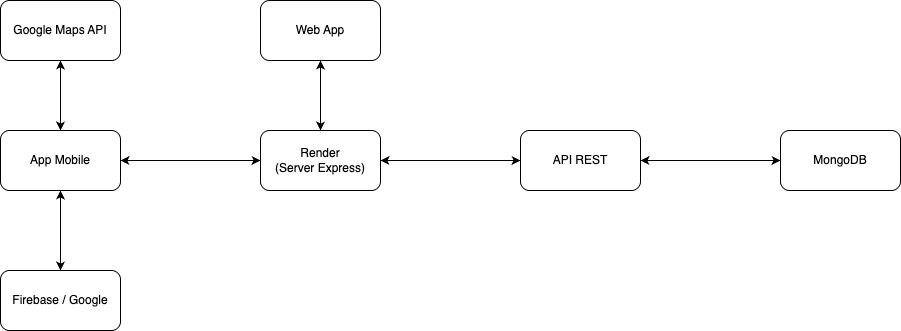
\includegraphics[width=1\linewidth]{D4-G1/Img/Diagramma Deploy.png}
    \caption{Diagramma di Deploy}
    \label{fig:enter-label}
\end{figure}
\begin{itemize}
    \item Componenti Interni: App Mobile, Web App, API REST, Database.
    \item Componenti Esterni: Servizi Firebase (Google), Servizio di geolocalizzazione (Google Maps API), Servizio di Hosting (Render), Servizio di database (MongoDB).
\end{itemize}

\subsection{Stack Tecnologico Utilizzato}
Il progetto è stato sviluppato utilizzando un \textbf{stack tecnologico} comprensivo di diverse tecnologie e metodologie. Ecco una panoramica delle tecnologie adottate:
\begin{itemize}
    \item Frontend:
    \begin{itemize}
        \item \textit{Mobile:} Flutter.
        \item \textit{Web:} HTML, CSS, JavaScript (Senza Framework).
    \end{itemize}
  \item Backend:
  \begin{itemize}
      \item \textit{API REST:} Node.js con Express.
      \item \textit{Documentazione API:} SwaggerAPI per generare e mantenere la documentazione delle API.
      \item \textit{Database:} MongoDB con Mongoose per la gestione dei dati.
      \item \textit{Autenticazione:} Login tramite Firebase. Google tramite Firebase per Login Terze Parti.
  \end{itemize}
  \item \textit{Hosting:} Render Hosting.
  \item Servizi Esterni:
  \begin{itemize}
      \item \textit{Geolocalizzazione:} Google Maps API.
  \end{itemize}
\end{itemize}

\subsection{Conclusioni Finali}
Al termine del secondo sprint, il progetto ha raggiunto una prima versione funzionale di alcuni moduli principali, come:
\begin{itemize}
    \item Un'app mobile con alcune funzionalità di base implementate.
    \item Una web app semplice per la gestione amministrativa.
    \item Un backend con API REST documentate e integrate con un database MongoDB.
\end{itemize}

Tuttavia, il sistema è ancora incompleto e necessita di ulteriori sviluppi. Molte funzionalità sono state implementate solo parzialmente e ci sono margini significativi per miglioramenti in termini di usabilità, performance e scalabilità.

In futuro, sarebbe interessante:
\begin{itemize}
    \item Completare le funzionalità mancanti e migliorare quelle esistenti.
    \item Effettuare test approfonditi per individuare e correggere bug.
    \item Ottimizzare il sistema per gestire un carico maggiore di utenti.
\end{itemize}

In conclusione, il progetto rappresenta un'esperienza formativa significativa e il nostro obiettivo principale è stato quello di imparare e mettere in pratica le nuove tecnologie implementate.

\subsubsection{Note finali}
Si segnala che, nelle prime fasi di sviluppo, alcuni endpoint delle API sono stati denominati al singolare (es. /api/tipoRifiuto, /api/tipoSensore). Successivamente, per coerenza e best practice REST, sarebbe stato opportuno utilizzare la forma plurale (es. /api/tipiRifiuto, /api/tipiSensore). Tuttavia, per evitare refactoring e problemi di compatibilità, i nomi degli endpoint sono stati mantenuti invariati. Siamo consapevoli che la convenzione corretta prevede l’uso del plurale per le risorse REST.